\documentclass[12pt]{article}
\usepackage[letterpaper,margin=0.62in,headheight=15pt,headsep=15pt,footskip=25pt]{geometry}
\usepackage[T1]{fontenc}
\usepackage{helvet}
\renewcommand{\familydefault}{\sfdefault}
\usepackage{tikz}
\usetikzlibrary{arrows.meta}
\usepackage{fancyhdr}
\usepackage{array}
\pagestyle{fancy}
\fancyhf{}
\renewcommand{\headrulewidth}{0.35pt}
\fancyfoot[C]{\fontsize{9}{11}\selectfont Bellingham Math Circle / Week 15 / W15-RV-v1 / \thepage}
\renewcommand{\footrulewidth}{0pt}
\setlength{\parindent}{0pt}
\setlength{\parskip}{9pt}
\newcommand{\pageheader}[2]{\fancyhead[C]{\fontsize{11.5}{14}\selectfont Week 15 / #1 / #2}}
\newcommand{\problem}[2]{\textbf{Problem #1:} #2\par}
\newcommand{\site}[4]{\fill (#1,#2) circle[radius=0.065in];\node[anchor=#4,font=\large,inner sep=0pt,outer sep=5.5pt] at (#1,#2) {#3};}
\newcommand{\recordtable}{%
  \renewcommand{\arraystretch}{1.8}
  \begin{tabular}{|p{2.85in}|p{2.85in}|}\hline
  Place & Distance to its nearest black dot\\\hline
  & \\\hline
  & \\\hline
  & \\\hline
  & \\\hline
  \end{tabular}}
\begin{document}
\fontsize{14}{17.5}\selectfont

\pageheader{Farthest dots}{Grades K--1 and up}
Use string to compare straight-line distances. A tie gets all tied letters.
The map continues beyond the frame.

\problem{1}{Mark and label places with the letter of the dot farthest away. Can each dot be farthest from somewhere?}

\vspace{0.12in}
\begin{center}
\begin{tikzpicture}[x=0.75in,y=0.75in]
  \draw[gray!60,line width=0.6pt] (-3,-3) rectangle (3,3);
  \site{-2}{-2}{A}{north east}
  \site{2}{-2}{B}{north west}
  \site{2}{2}{C}{south west}
  \site{-2}{2}{D}{south east}
  \site{0}{0}{E}{south west}
\end{tikzpicture}
\end{center}
\vspace{0.08in}
\rule{\linewidth}{0.35pt}
\par\vspace{0.32in}
\rule{\linewidth}{0.35pt}
\par\vspace{0.32in}
\rule{\linewidth}{0.35pt}

\newpage
\pageheader{Grid-step distance}{Grades 2--3 and up}
Travel horizontally or vertically from any point, including inside squares. One grid edge is one step; a fraction of an edge is that fraction of a step. Distance is the length of a shortest trip. A tie gets both letters. The grid continues beyond the frame.

\begin{center}
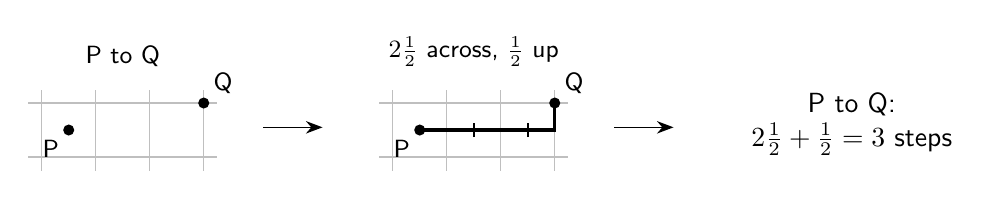
\begin{tikzpicture}[x=0.27in,y=0.27in,font=\small]
  \begin{scope}
    \node[anchor=south] at (1.5,1.5) {P to Q};
    \draw[step=1,gray!50] (-0.25,-0.25) grid (3.25,1.25);
    \fill (0.5,0.5) circle[radius=2pt]; \node[anchor=north east] at (0.5,0.5) {P};
    \fill (3,1) circle[radius=2pt]; \node[anchor=south west] at (3,1) {Q};
  \end{scope}
  \draw[-{Stealth[length=6pt]},line width=0.6pt] (4.1,0.55)--(5.2,0.55);
  \begin{scope}[shift={(6.5,0)}]
    \node[anchor=south] at (1.5,1.5) {$2\frac12$ across, $\frac12$ up};
    \draw[step=1,gray!50] (-0.25,-0.25) grid (3.25,1.25);
    \draw[line width=1.2pt] (0.5,0.5)--(3,0.5)--(3,1);
    \foreach \x in {1.5,2.5}{\draw[line width=0.8pt] (\x,0.37)--(\x,0.63);}
    \fill (0.5,0.5) circle[radius=2pt]; \node[anchor=north east] at (0.5,0.5) {P};
    \fill (3,1) circle[radius=2pt]; \node[anchor=south west] at (3,1) {Q};
  \end{scope}
  \draw[-{Stealth[length=6pt]},line width=0.6pt] (10.6,0.55)--(11.7,0.55);
  \node[align=center,font=\normalsize] at (15,0.6) {P to Q:\\$2\frac12+\frac12=3$ steps};
\end{tikzpicture}
\end{center}

\problem{2}{Label grid crossings A, B, or AB for the nearer dot. Do ties fill whole small squares? Can two tied places have a midpoint that is not tied?}

\begin{center}
\begin{tikzpicture}[x=0.5625in,y=0.5625in]
  \draw[step=1,gray!50,line width=0.35pt] (-2,-2) grid (6,6);
  \draw[gray!65,line width=0.6pt] (-2,-2) rectangle (6,6);
  \fill (0,0) circle[radius=0.065in];
  \node[anchor=north east,font=\large,inner sep=0pt,outer sep=5.5pt] at (0,0) {A};
  \fill (2,2) circle[radius=0.065in];
  \node[anchor=south west,font=\large,inner sep=0pt,outer sep=5.5pt] at (2,2) {B};
\end{tikzpicture}
\end{center}
\rule{\linewidth}{0.35pt}
\par\vspace{0.3in}
\rule{\linewidth}{0.35pt}

\newpage
\pageheader{Largest nearest distance}{Grades 4--5}
For Problems 3 and 4, use straight-line distances. New points must stay inside or on the square. If nearest dots tie, their shared distance counts.

\problem{3}{Put a new point in the square so its distance to the nearest black dot is as large as possible. Find every best place, and explain why no other place is better.}

\begin{center}
\begin{tikzpicture}[x=1.125in,y=1.125in]
  \draw[line width=0.8pt] (-2,-2) rectangle (2,2);
  \site{-2}{-2}{A}{north east}
  \site{2}{-2}{B}{north west}
  \site{2}{2}{C}{south west}
  \site{-2}{2}{D}{south east}
\end{tikzpicture}
\end{center}
\vspace{0.05in}
\begin{center}\recordtable\end{center}
\vspace{0.15in}
\rule{\linewidth}{0.35pt}

\newpage
\pageheader{Largest nearest distance}{Grades 4--5}
\problem{4}{The center is now a black dot too. Find every best place in the square, and explain why no other place has a larger distance to its nearest black dot.}

\vspace{0.08in}
\begin{center}
\begin{tikzpicture}[x=1.125in,y=1.125in]
  \draw[line width=0.8pt] (-2,-2) rectangle (2,2);
  \site{-2}{-2}{A}{north east}
  \site{2}{-2}{B}{north west}
  \site{2}{2}{C}{south west}
  \site{-2}{2}{D}{south east}
  \site{0}{0}{E}{south west}
\end{tikzpicture}
\end{center}
\vspace{0.15in}
\begin{center}\recordtable\end{center}
\vspace{0.25in}
\rule{\linewidth}{0.35pt}
\par\vspace{0.3in}
\rule{\linewidth}{0.35pt}
\end{document}
